\documentclass[a4paper]{article}
\usepackage{graphicx}
\usepackage[ngerman]{babel}

\begin{document}
\section*{Invertierender Operationsverst\"arker}
d)\\
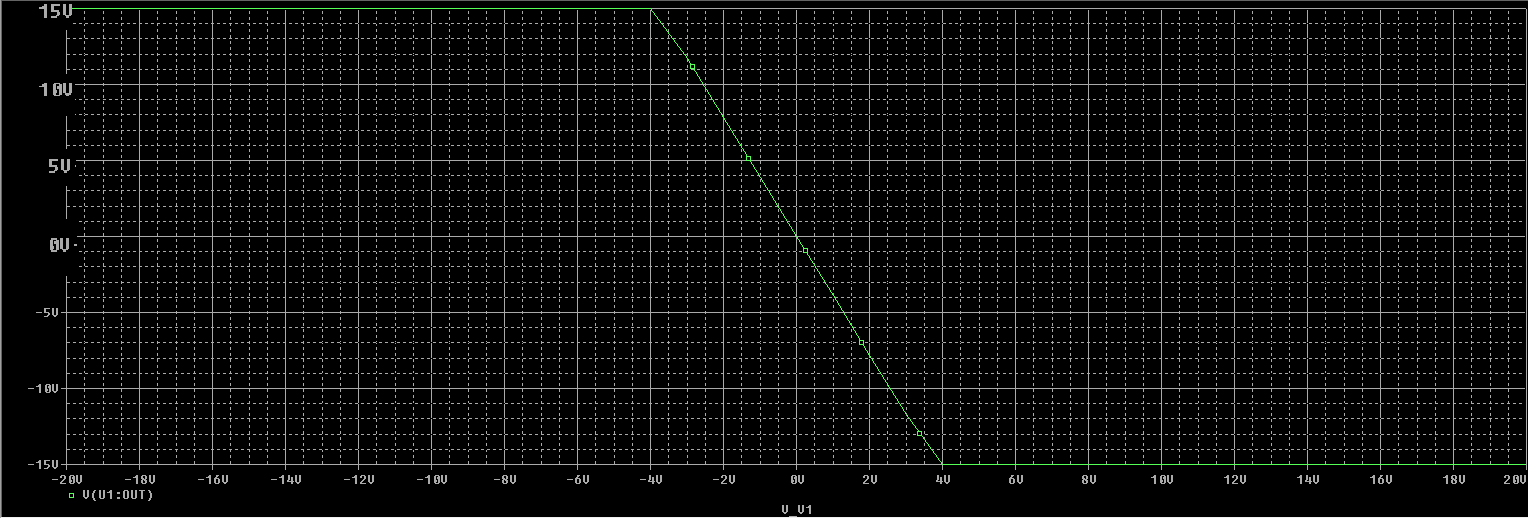
\includegraphics[scale=0.4]{SimulationInverter_d}
\\[0.5cm]
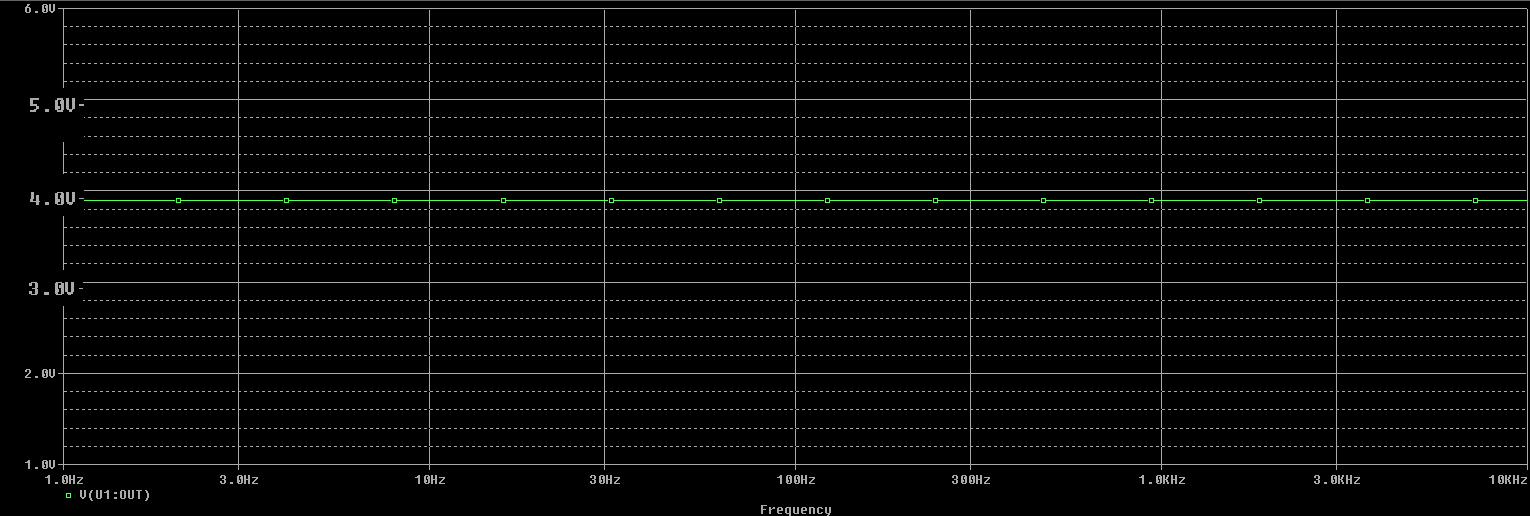
\includegraphics[scale=0.4]{SimulationInverterAC_d}
\newpage
\section*{Nichtinvertierender Operationsverst\"arker}
e)\\
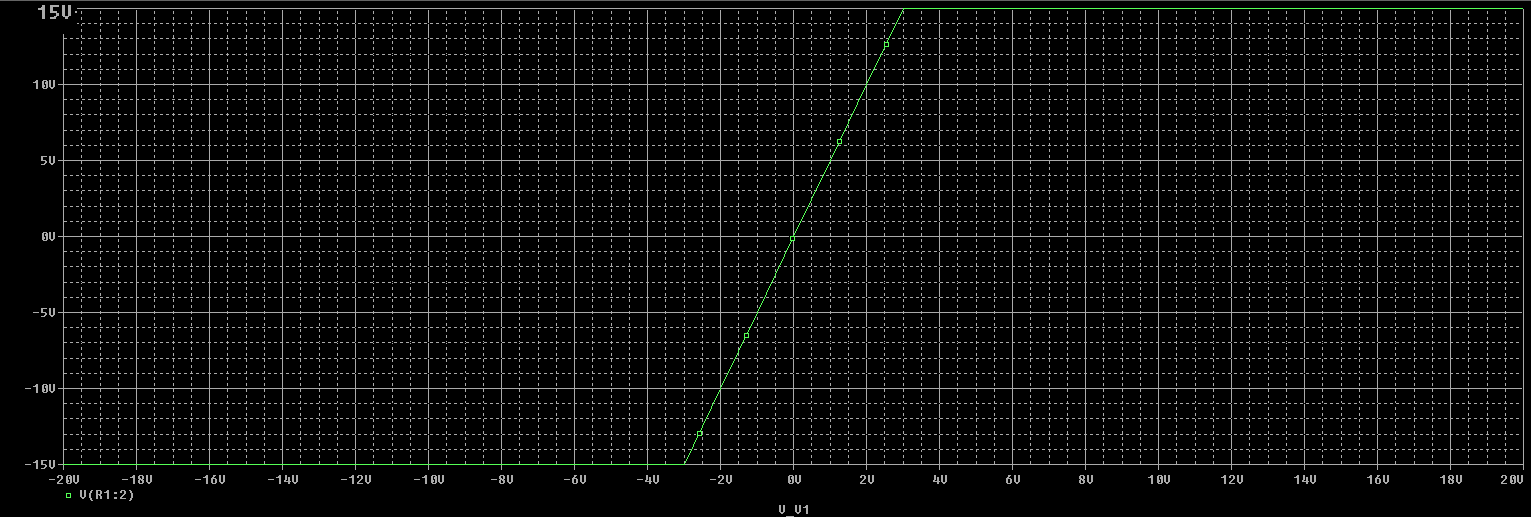
\includegraphics[scale=0.4]{SimulationNichtInverter_e}
\\[0.5cm]
f) \\
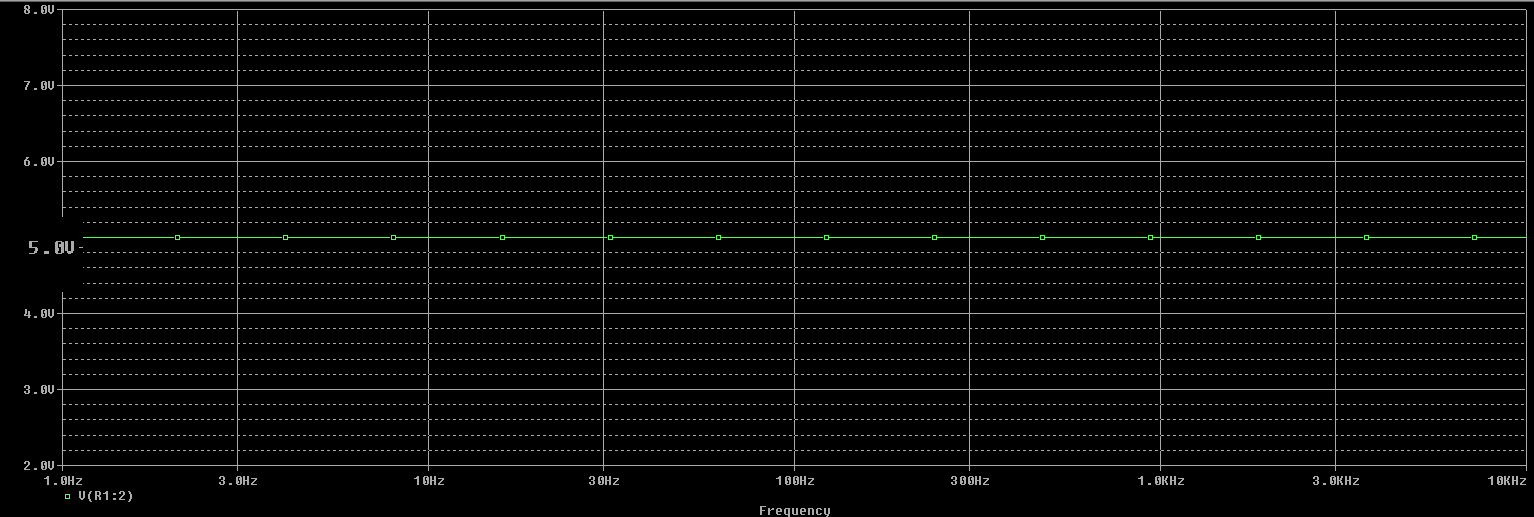
\includegraphics[scale=0.4]{SimulationNichtInverterAC_e}
g) \\
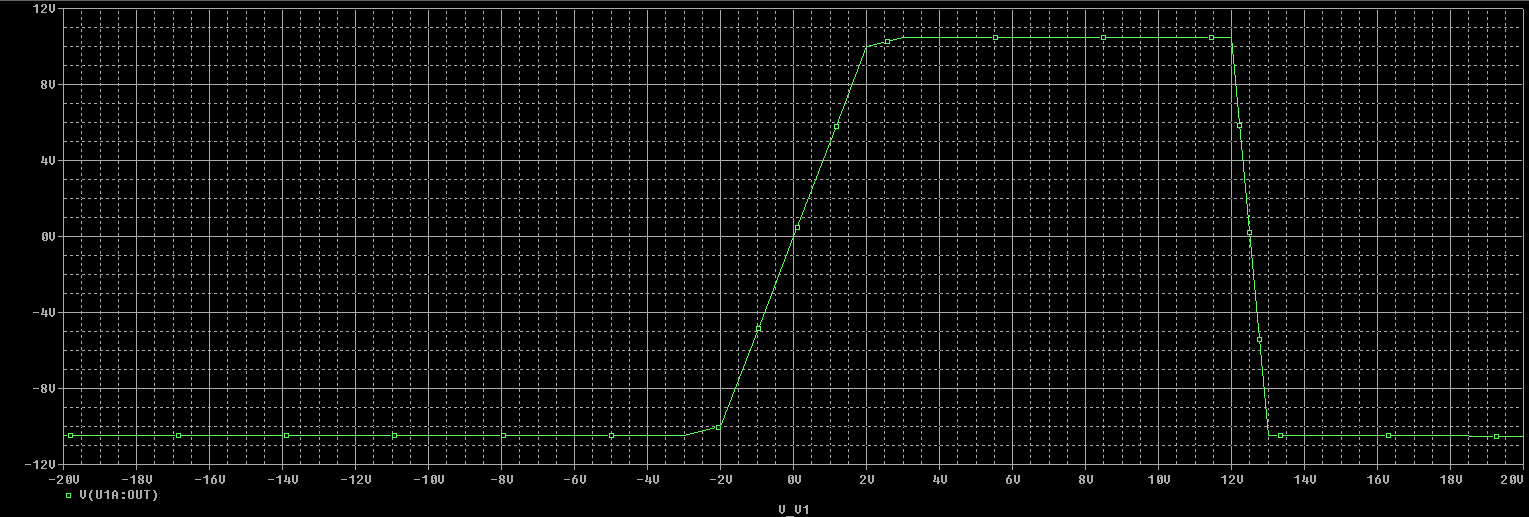
\includegraphics[scale=0.4]{SimulationNichtInverterAC_Real_f}
h) \\
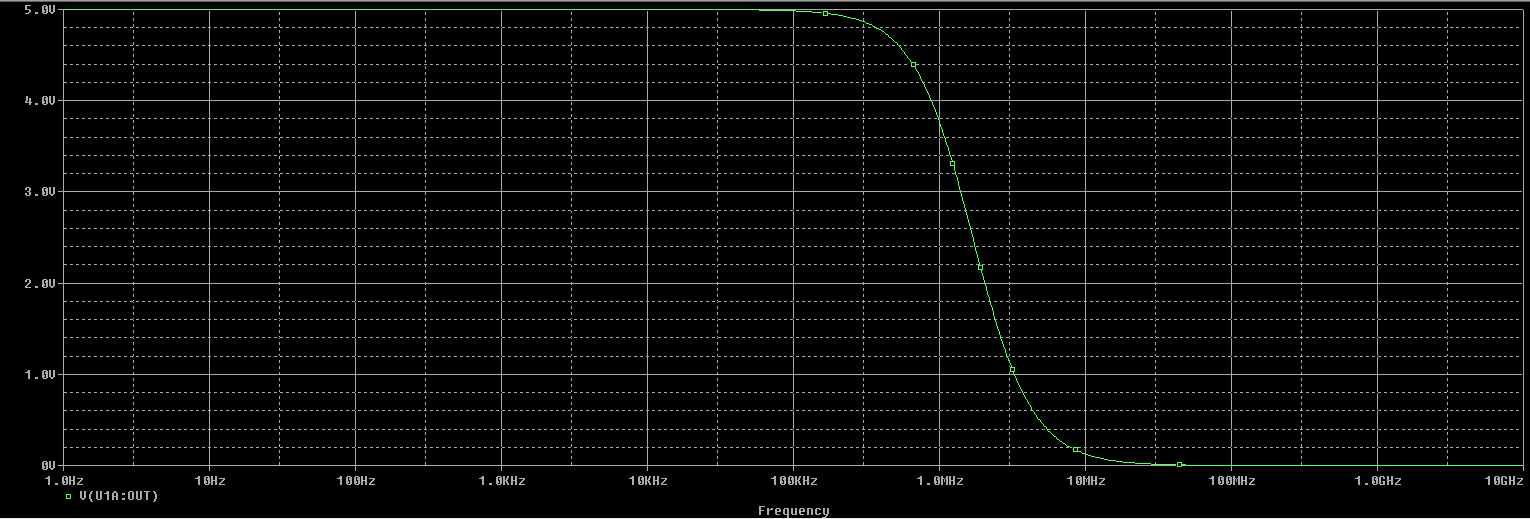
\includegraphics[scale=0.4]{SimulationNichtInverterAC_Real_h_5}
\\[0.5cm]
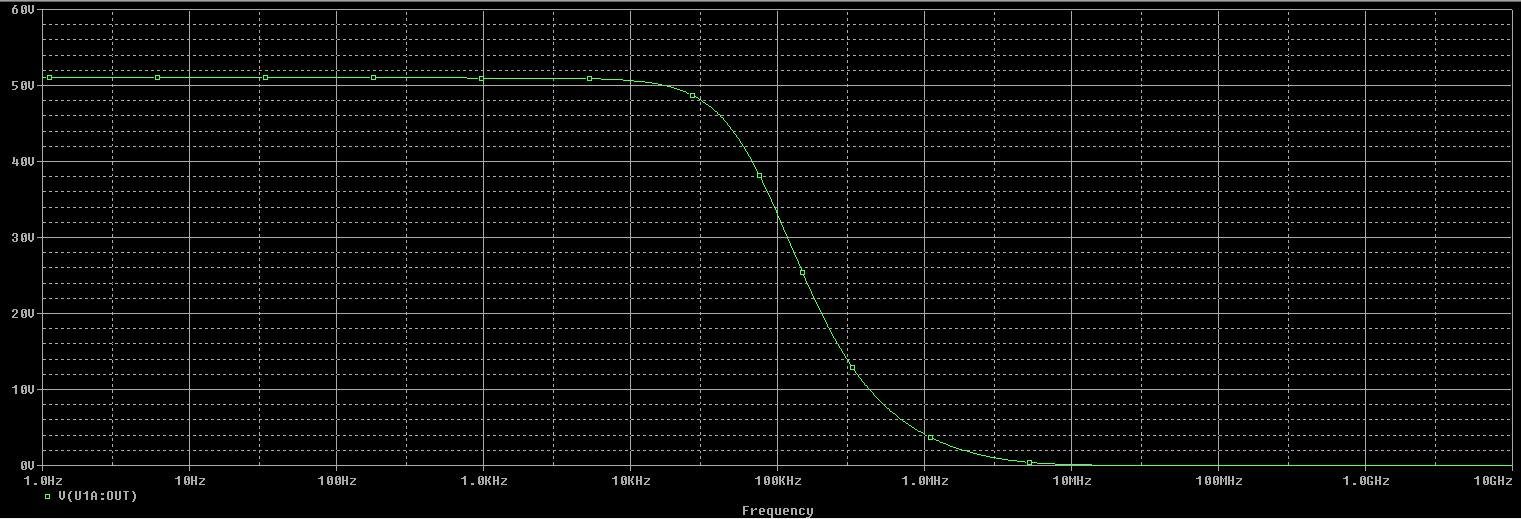
\includegraphics[scale=0.4]{SimulationNichtInverterAC_Real_h_50}

\section*{Hochohmige Spannungsquelle}
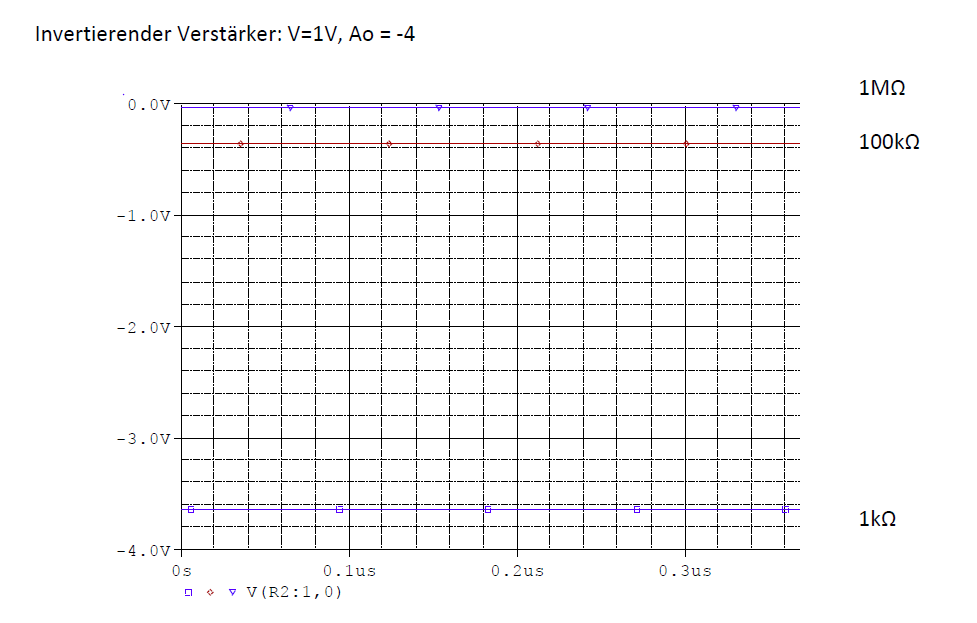
\includegraphics[scale=0.6]{SimulationInverter_a)}
\\[0.5cm]
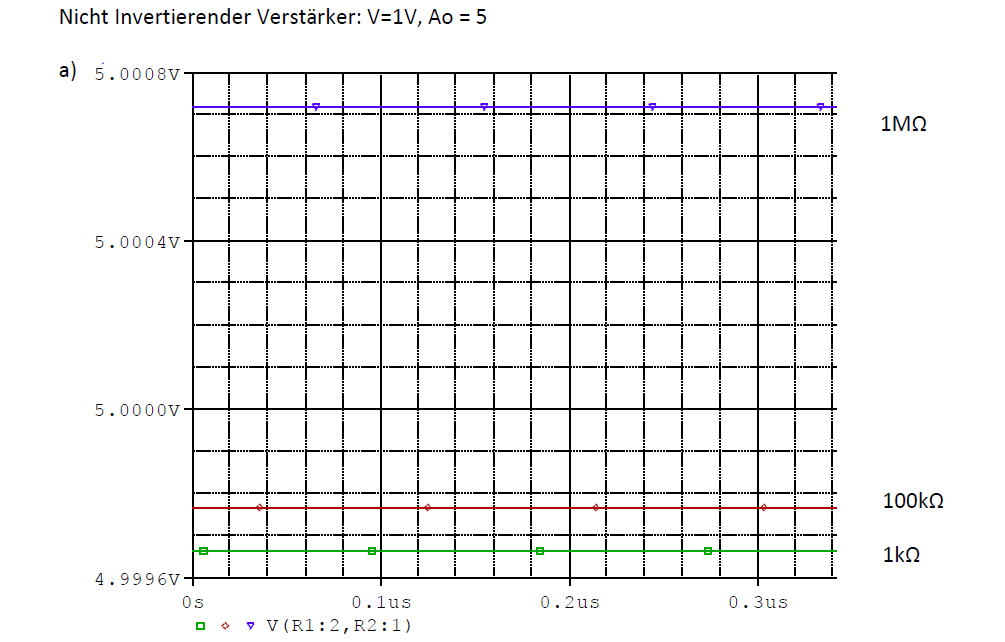
\includegraphics[scale=0.6]{SimulationInverter_a)_1}
\end{document}